%\subsubsection{The \emph{Challenger} disaster}
\begin{Example}[nasa]{Challenger disaster}
\ixd{Challenger disaster|(}
\begin{changebar}
The space shuttle \emph{Challenger} exploded 73 seconds after take-off on
\end{changebar} 
January 28, 1986.
Subsequent investigation determined that the cause was failure of the O-ring
seals used to isolate the fuel supply from burning gases.
The story behind the \emph{Challenger} disaster is perhaps the most poignant
missed opportunity in the history of statistical graphics.
It may be heartbreaking to find out that some important information
was there, but the graph maker missed it.

Engineers from Morton Thiokol, manufacturers of the rocket motors,
had been worried about the effects of unseasonably cold weather
on the O-ring seals and recommended aborting the flight.
NASA staff analysed the data on the relation between ambient temperature
and the number of O-ring failures (out of 6), but they had excluded observations
where no O-rings failed,
believing that they were uninformative.
Unfortunately, those observations had occurred when the launch temperature
was relatively warm (\degree{65-80}F.) and were indeed informative.
The coldest temperature at any previous launch was \degree{53};  when \emph{Challenger} was launched on January 28,
the temperature was a frigid \degree{31}.

The data relating O-ring failures to temperature were depicted as in
\figref{fig:nasa0}, our candidate for the most misleading graph of history.
Examination of this graph seemed to indicate that there was no relation
between ambient temperature and failure.  Thus, the decision to launch
the \emph{Challenger} was made, in spite of the initial concerns
of the Morton Thiokol engineers.
\begin{figure}[htb]
  \centering
  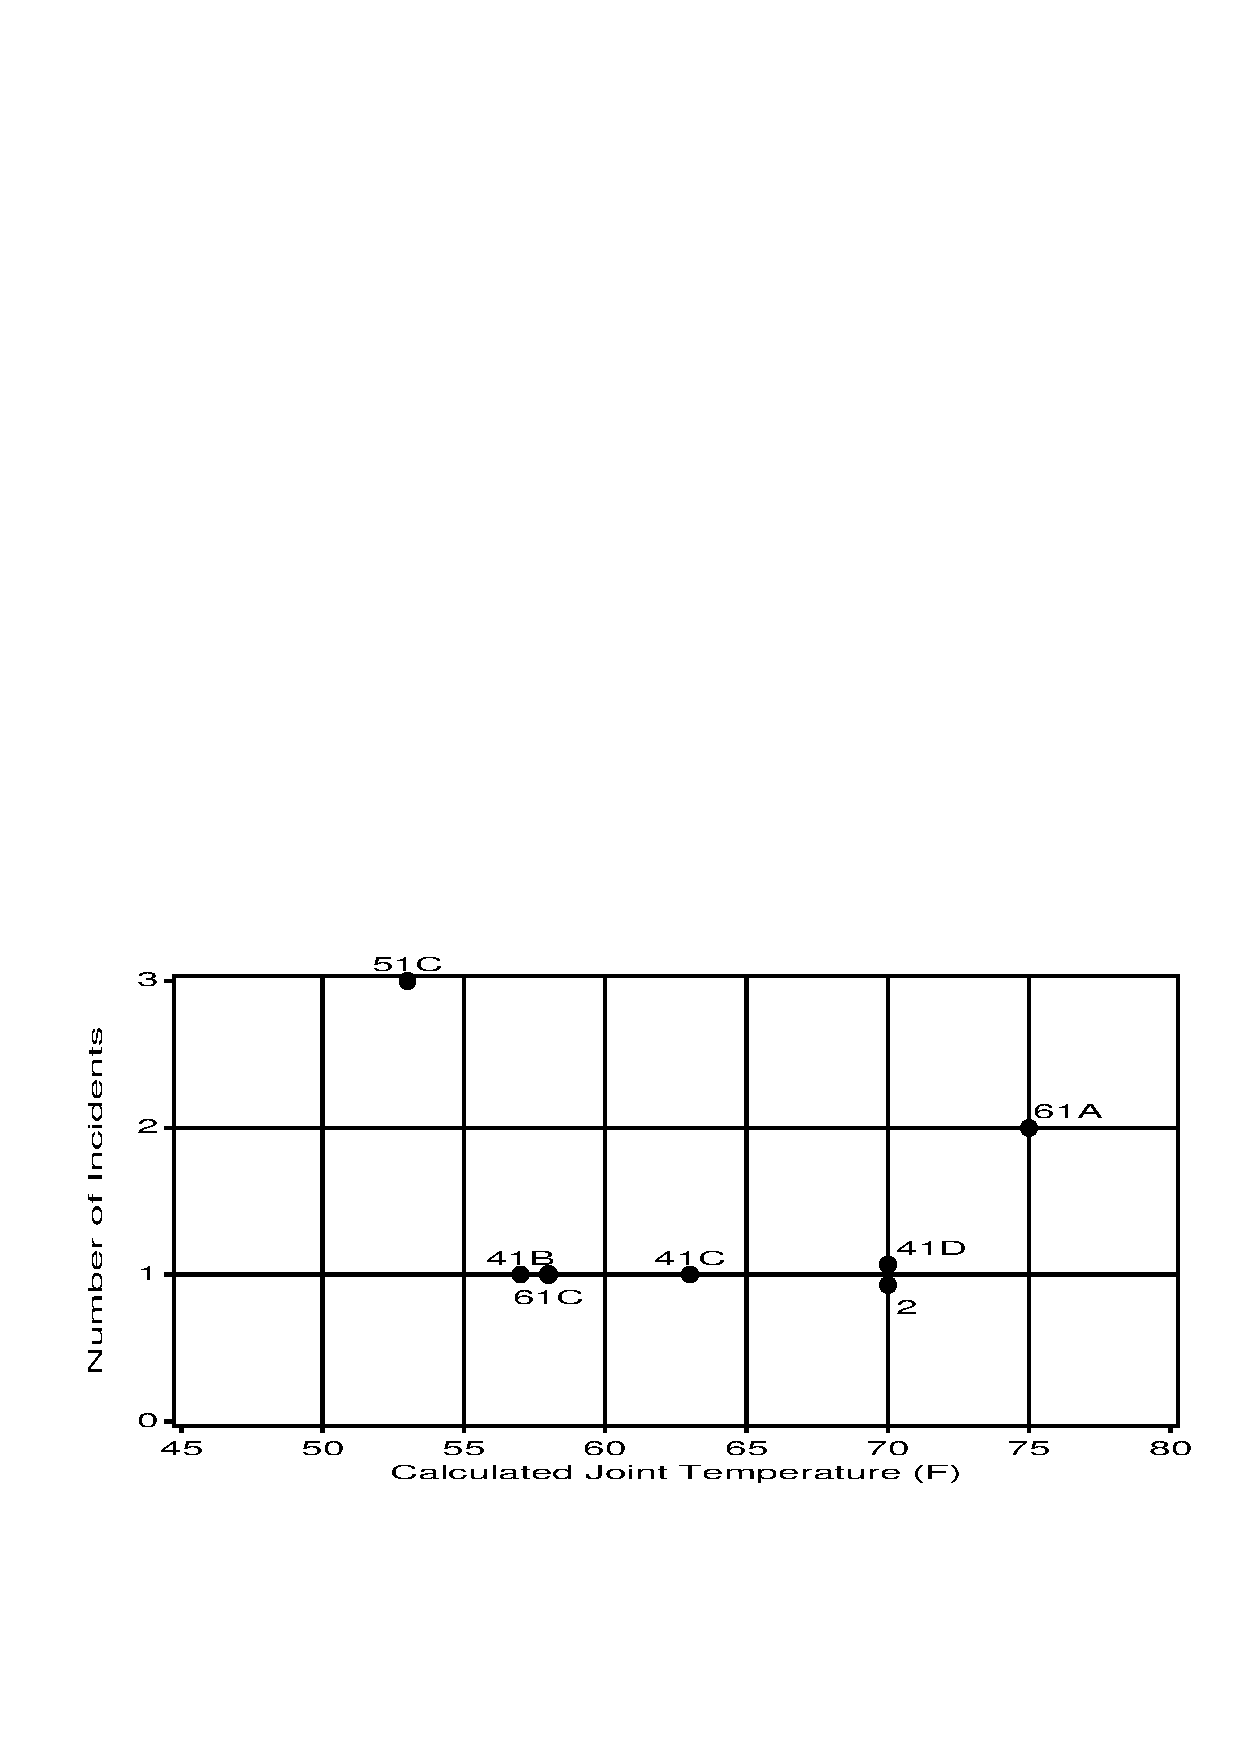
\includegraphics[width=\textwidth,clip]{ch6/fig/nasa0}
  \caption{NASA Space Shuttle pre-launch graph}\label{fig:nasa0}
\end{figure}

These data have been analyzed extensively
\citep{Dalal-etal:89,Lavine:91}.
\citet{Tufte:97} gives a thorough and convincing
visual analysis of the evidence available prior to the launch.
The main goal here is to
illustrate predictions from the model for the \emph{Challenger} launch
and graphical display.
But, what if the engineers had simply made a better graph?
At the least, that would entail
\begin{seriate}
\item drawing a smoothed curve to fit the points (to show the trend)
\item removing the background grid lines (which obscure the data).
\end{seriate}
\figref{fig:nasa02} 
shows a revised version of the same 
graph, which should have caused any engineer to conclude that
either 
\begin{seriate}
\item the data were wrong, or
\item there were excessive risks
associated with both high and low temperatures.
\end{seriate}
But it is well-known
that brittleness of the rubber used in the O-rings is inversely
proportional to $(\texttt{temp})^3$, so prudent interest might have focussed
on the first possibility.

\begin{figure}[htb]
  \centering
  \includegraphics[clip,width=\textwidth]{ch6/fig/nasa02}
  \caption{NASA Space Shuttle pre-launch graph, revised}\label{fig:nasa02}
\end{figure}

We return to the problem of predicting the likelihood of failures at
low temperatures.
The \Dstp{} below reads the data on the number of O-ring failures
and temperature for the 23 flights for which information was available
before the \emph{Challenger} launch.  A more detailed \Dset,
from \citet{Dalal-etal:89} and \citet{Tufte:97} is given in \datref{dat:orings}.

\begin{listing}
title 'NASA Space Shuttle O-Ring Failures';
data nasa;
   input failures temp @@;
   orings = 6;
   label failures = 'Number of O-ring failures'
      temp = 'Temperature (deg F)';
   datalines;
   2  53    1  57    1  58     1  63
   0  66    0  67    0  67     0  67
   0  68    0  69    0  70     0  70
   1  70    1  70    0  72     0  73
   0  75    2  75    0  76     0  76
   0  78    0  79    0  80
;
\end{listing}
To obtain predicted probabilities for observations not in the original sample,
create an additional \Dset\ which contains values for the independent
variables in the extrapolation sample, and join these observations to the
actual \Dset.  The response variable (\texttt{failures}) will be missing
for the extrapolation sample.

\begin{listing}
*-- Obtain predicted values for 30-80 degrees;
data temp;
   input temp @@;
datalines;
31 30 35 40 45 50 55 60 65 70 75 80
;
data nasa2;
   set nasa temp;
\end{listing}
In the \PROC{LOGISTIC} step, we use the \boldital{events/trials} syntax
to indicate the number of failures and number of trials.
(This does assume that O-rings on the same flight fail independently.)
The observations in the extrapolation sample are not used in fitting
the model, yet the procedure produces predicted probabilities and
logits (as long as the independent variable(s) are non-missing).

\begin{listing}
proc logistic data=nasa2 nosimple;
   model failures/orings = temp ;
   output out=results p=predict l=lower u=upper;
proc print;
\end{listing}
The printed output, shown in \outref{out:nasa.1} indicates that the
12 new observations were not used in the analysis.
The odds ratio, 0.891, is interpreted to mean that each increase of
\degree{1} in temperature decreases the odds of a failure by 11\%!

\begin{Output}[htbp]
\caption{Logistic regression for NASA O-ring data}\label{out:nasa.1}
\small
\verbatiminput{ch6/out/nasa.1}
\end{Output}

The \ODS\ \pname{results} contains the predicted probability
of a failure of a single O-ring
at each temperature and upper and lower confidence 95\% limits
for this probability.  We can plot the predicted and observed values
as shown below.  A vertical reference line at \degree{31} is used
to highlight the conditions at the \emph{Challenger} launch.
\begin{listing}
proc sort data=results;
   by predict;
data results;
   set results;
   obs = failures / orings;

proc gplot data=results;
   plot (obs predict lower upper) * temp /
      href=31 lhref=33
      overlay frame vaxis=axis1 vminor=1;
   symbol1 v=dot i=none c=blue h=2;
   symbol2 v=none i=spline c=black w=5;
   symbol3 v=none i=spline c=red l=33 r=2 w=3;
   axis1 label=(a=90 'Estimated Failure probability') offset=(3);
\end{listing}

The graph is shown in \figref{fig:nasa}.  There's hardly any data
at low temperatures and the width of the confidence band provides
an important visual cue to this uncertainty. Nevertheless,
the predicted probability of failure per O-ring is uncomfortably
 high at \emph{all} temperatures below the range of data from
previous flights.  Would you take a ride on \emph{Challenger} when
the weather is cold?

\begin{figure}[htb]
  \centering
  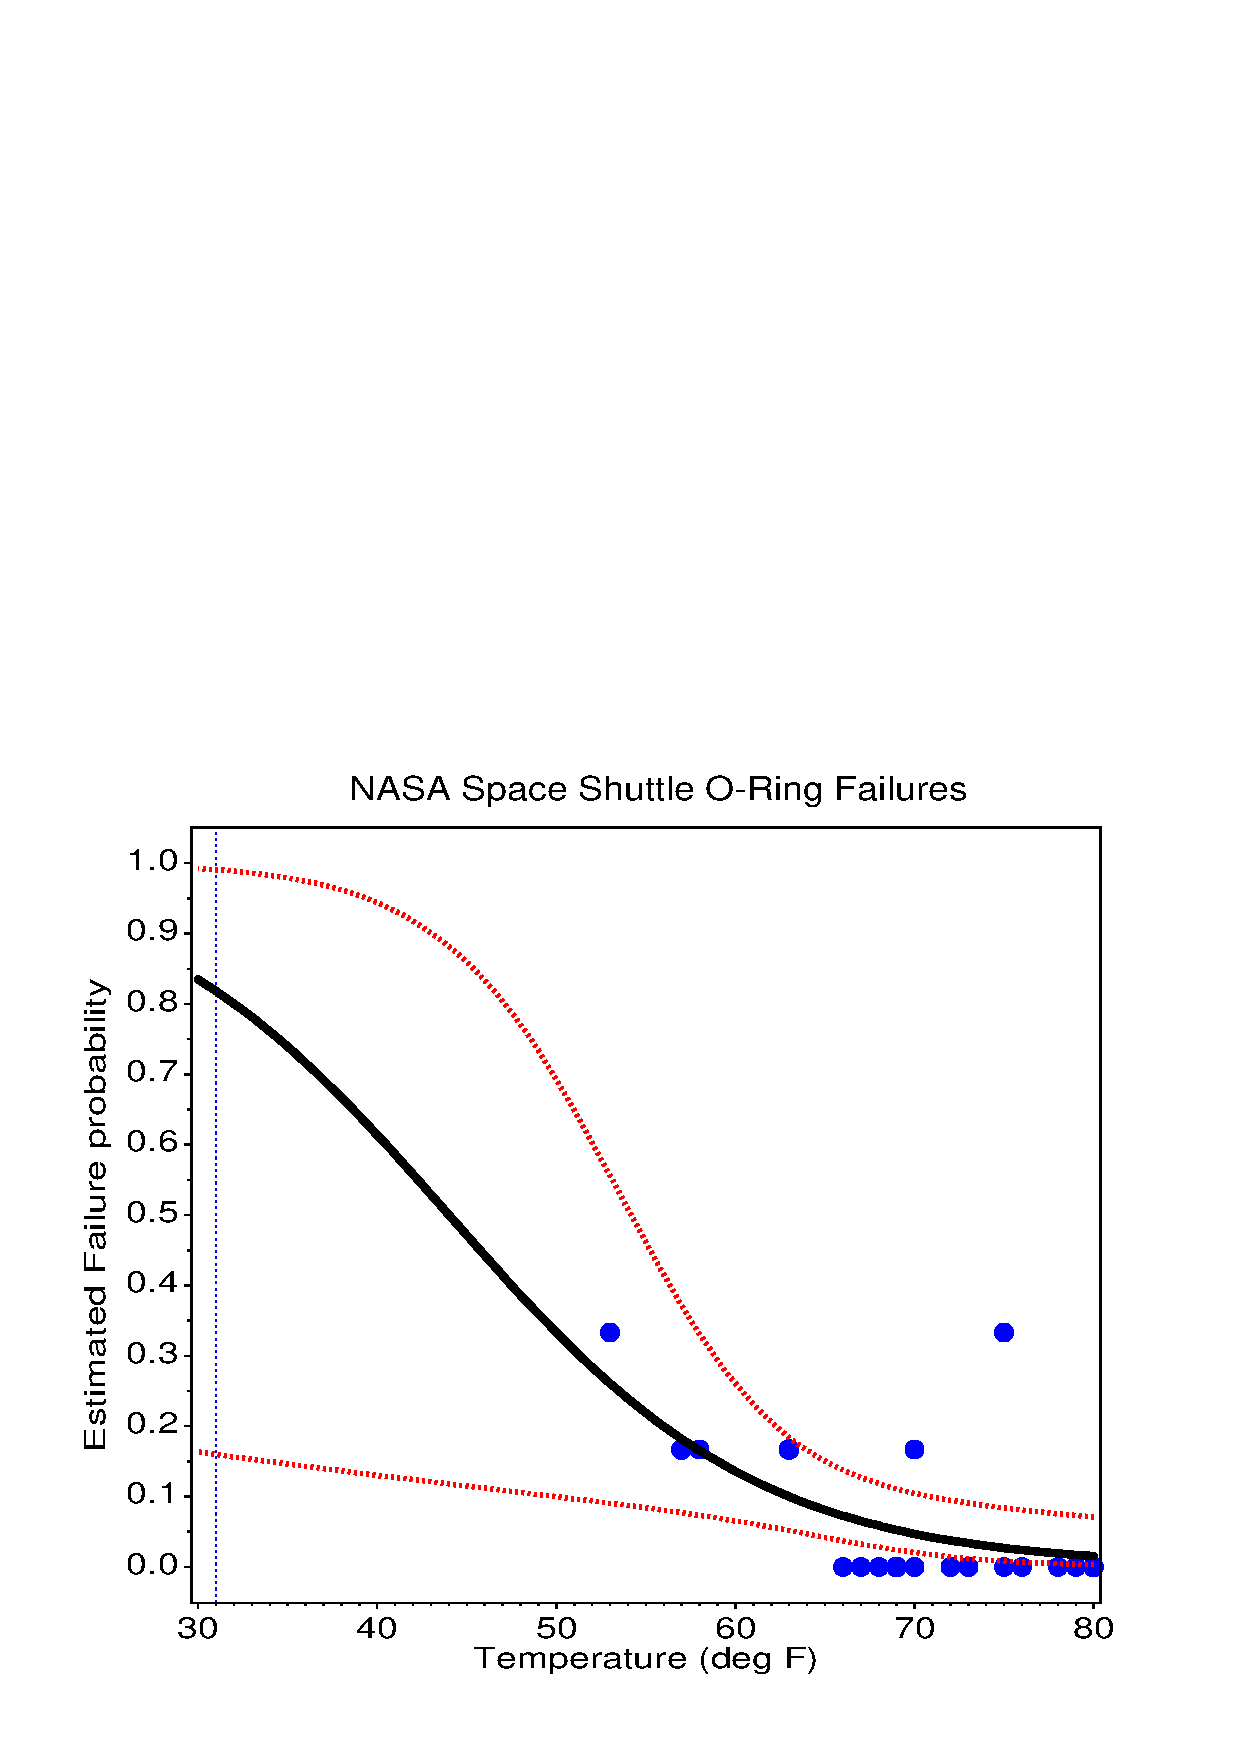
\includegraphics[scale=.75]{ch6/fig/nasa}
  \caption{NASA Space Shuttle O-ring Failure, Observed and Predicted probabilities}\label{fig:nasa}
\end{figure}
\ixd{Challenger disaster|)}
\end{Example}
